\documentclass[pdflatex]{sn-jnl}
 \renewcommand{\textfraction}{.002}
\renewcommand{\floatpagefraction}{.995}
\setcounter{totalnumber}{5}
\renewcommand{\topfraction}{.995}

\usepackage[numbers,square]{natbib}
\bibliographystyle{spbasic_u}

\usepackage[noend,ruled,vlined]{algorithm2e}
\newcommand\mycommfont[1]{\footnotesize\ttfamily{#1}}
\SetCommentSty{mycommfont}


\usepackage{graphicx}%
\usepackage{multirow}%
\usepackage{amsmath,amssymb,amsfonts}%
\usepackage{amsthm}%
\usepackage{mathrsfs}%
\usepackage[title]{appendix}%
\usepackage{xcolor}%
\usepackage{textcomp}%
\usepackage{manyfoot}%
\usepackage{booktabs}%
\usepackage{placeins}
\usepackage{listings}%
\usepackage{mathtools}
\usepackage{subcaption}
\usepackage{xr}
\usepackage{bm}
%% CUSTOM PACKAGES
%\usepackage[linesnumbered,ruled,vlined]{algorithm2e}
\usepackage{hyperref}
\usepackage{array}
\usepackage{tabularx}
\usepackage{tikz}
\usetikzlibrary{shapes.geometric}
%\usetikzlibrary{3d,perspective}
%\usetikzlibrary{shapes.geometric, arrows.meta, positioning}
\usepackage{booktabs} % For better table lines
\usepackage[version=4]{mhchem} 
\usepackage{enumitem}
\usepackage{algorithm2e}
%\usepackage{arydshln}

%%%%%%%%%%%%%%%%%%%%%%%%%%%%%%%%%%%%%%%%%%%%%%%%%%%%%%%%%%%%%%%%%%%%%%%%%%%

%% as per the requirement new theorem styles can be included as shown below
\theoremstyle{thmstyleone}%
\newtheorem{theorem}{Theorem}%  meant for continuous numbers
\newtheorem{corollary}[theorem]{Corollary}% 
\newtheorem{proposition}[theorem]{Proposition}%
\newtheorem{lemma}[theorem]{Lemma}% 
\newtheorem{conjecture}[theorem]{Conjecture}%
\newtheorem{observation}[theorem]{Observation}%
%
\makeatletter
\newtheoremstyle{examplesty}% Numbered
{18pt plus2pt minus1pt}% Space above
{18pt plus2pt minus1pt}% Space below
{\normalfont}% Body font
{0pt}% Indent amount
{\bfseries}% Theorem head font
{.}% Punctuation after theorem head
{.5em}% Space after theorem headi
{\thmname{#1}\thmnumber{\@ifnotempty{#1}{ }{#2}}%
  \thmnote{ {\the\thm@notefont(#3)}}}% Theorem head spec (can be left empty, meaning `normal')
\makeatother
\theoremstyle{examplesty}%
\newtheorem{example}{Example}%
%\newtheorem{remark}{Remark}%
%
\theoremstyle{thmstylethree}%
\newtheorem{definition}[theorem]{Definition}%

\newenvironment{mainitem}[2]{\medskip\par\noindent%
  \textbf{#1~M\ref{#2}.}}{\par}


%%%%% SOME LOW LEVEL STUFF NEEDED FOR SPECIAL SYMBOLS
\makeatletter
\def\moverlay{\mathpalette\mov@rlay}
\def\mov@rlay#1#2{\leavevmode\vtop{%
    \baselineskip\z@skip \lineskiplimit-\maxdimen
    \ialign{\hfil$\m@th#1##$\hfil\cr#2\crcr}}}
\newcommand{\charfusion}[3][\mathord]{
  #1{\ifx#1\mathop\vphantom{#2}\fi
    \mathpalette\mov@rlay{#2\cr#3}
  }
  \ifx#1\mathop\expandafter\displaylimits\fi}
\DeclareRobustCommand\bigop[1]{%
  \mathop{\vphantom{\sum}\mathpalette\bigop@{#1}}\slimits@
}
\newcommand{\bigop@}[2]{%
  \vcenter{%
    \sbox\z@{$#1\sum$}%
    \hbox{\resizebox{\ifx#1\displaystyle.9\fi\dimexpr\ht\z@+\dp\z@}{!}{$\m@th#2$
}}%
  }%
}
\makeatother
%%%%% END LOWLEVEL USER DEFINITION

\newcommand{\cupdot}{\charfusion[\mathbin]{\cup}{\cdot}}
\DeclareMathOperator{\bigcupdot}{\charfusion[\mathop]{\bigcup}{\cdot}}
% \DeclareMathOperator{\Aut}{Aut}
% \DeclareMathOperator{\orb}{orb}
\newcommand{\whatever}{\mbox{\,.\,}}
\newcommand{\king}{K}
\newcommand{\queen}{\mathbf{Q}}
\newcommand{\prince}{\mathbf{P}}
\newcommand{\food}{\ensuremath{\mathbf{F}}}
\newcommand{\SM}{\mathbb{S}}
\newcommand{\closure}[2]{\mathscr{C}_{#1}(#2)}
\newcommand{\cl}[0]{c}
\newcommand{\CR}[0]{\mathcal{R}}
\newcommand{\C}[1]{\mathit{#1}}
\newcommand{\FR}[0]{\mathbf{R}}
%\newcommand{\F}[1]{\mathbf{#1}}
\newcommand{\fr}[0]{\mathbf{r}}
\newcommand{\net}[1]{\hat{#1}}
\newcommand{\RAF}[0]{\mathbf{R}'}
\newcommand{\PO}[0]{d}
\newcommand{\POR}[0]{\mathscr{R}}
\newcommand{\POX}[0]{\mathscr{X}}
\newcommand{\cat}{\mathbf{C}}
\newcommand{\sgen}{g}
\newcommand{\rgen}{\gamma}
\newcommand{\ceducts}{\mathcal{E}}
\newcommand{\cproducts}{\mathcal{P}}
\newcommand{\feducts}{\mathbf{E}}
\newcommand{\fproducts}{\mathbf{P}}
\newcommand{\ORCID}[1]{}
\DeclareMathOperator{\suck}{succ}
\newcommand{\Code}[1]{\texttt{\upshape{#1}}}
\newcommand{\pfad}[0]{\ensuremath{\mathbf{P}}}
\newcommand{\stack}[0]{\ensuremath{\mathbf{T}}}
\newcommand{\child}{\pmb{\kappa}}

\definecolor{middlegreen}{RGB}{0,128,0}
\definecolor{royalpurple}{RGB}{85,26,139}
\newcommand{\NEW}[1]{\begingroup\color{blue}#1\endgroup}
\newcommand{\TODO}[1]{\begingroup\color{red}#1\endgroup}
\newcommand{\PFS}[1]{\begingroup\color{blue}#1\endgroup}
\newcommand{\holy}[1]{\begingroup\color{royalpurple}#1\endgroup}
\newcommand{\TG}[1]{\begingroup\color{green}#1\endgroup}
\newcommand{\NV}[1]{\begingroup\color{teal}#1\endgroup}
\newcommand{\OLD}[1]{\begingroup\tiny\color{gray}#1\endgroup}

% Linenumbers for debugging
\usepackage{lineno}
\linenumbers
\raggedbottom

%%%%%%%%%%%%%%%%%%%%%%%%%%%%%%%%%%%%%%%%%%%%%%%%%%%%%%%%%%%%%%%%%%%
%%%%%%%%%%%%%%%%%%%%%%%%%%%%%%%%%%%%%%%%%%%%%%%%%%%%%%%%%%%%%%%%%%%
%%%%%%%%%%%%%%%%%%%%%%%%%%%%%%%%%%%%%%%%%%%%%%%%%%%%%%%%%%%%%%%%%%%

\begin{document}

\title{RAF-Cores: Deadwood} 


\maketitle


\vspace{6pt}
\begin{lemma}
	Every $\fr\in \RAF$ has at least one reactant (F-reactant or F-catalyst) that is not in $\food$. For 
	$\fr\in \RAF: \rgen(\fr)=1$, this is an F-catalyst.
\end{lemma}
\begin{proof}
	 Assume this is not the case for an $\fr\in \RAF$. Then $\{\fr\}$ is a RAF which contradicts minimality
	 and non-triviality of $\RAF$.
\end{proof}

Since all food molecules are absent in $\queen''$, it contains an elementary circuit since all vertices have an 
in-degree greater than zero \cite{bang-jensen_digraphs_2002}. Since $\queen''\subseteq \queen'$ we obtain:
\vspace{6pt}
\begin{corollary}
	The graphs $\queen'$ and $\queen''$ contain an elementary circuit. 
\end{corollary}
\vspace{6pt}

In \cite{steel_minimal_2013} this was already shown for the reaction graph, but not for the bipartite graph. For minimal RAFs, this result 
can be strengthened to the statement that every reaction in $\queen'$ and $\queen''$ is located on an elementary circuit. We start by 
showing that each first-generation reaction is located on an elementary circuit. To this end, we define the descendants and ascendants 
of a vertex $v$ in a graph in the following way

\begin{equation}
	\begin{split}
		D(v) & \coloneqq \{u \in V \ | \text{ exists a path } P=(v,\ldots, u)  \} \\
		A(v) & \coloneqq \{u \in V \ | \text{ exists a path } P=(u,\ldots, v)  \} \\
	\end{split}
\end{equation}

\begin{lemma}
	Let $\RAF$ be a minimal, non-trivial RAF. Then every first-generation reaction 
	is located on an elementary circuit that is not a digon in $\queen'$ and $\queen''$.
\end{lemma}
\begin{proof}
	We start with $\queen''$ and assume this is not the case. Then there is a first-generation 
	reaction $\fr_1$, that has no incoming edges. Thus, all F-reactants and all F-catalysts are 
	in $\food$. Then $\{\fr_1\}$ is a RAF which directly contradicts that $\RAF$ is a non-trivial 
	and minimal RAF. Then $\fr_1$ has an incoming edge, and since $\rgen(\fr_1)=1$ all 
	F-reactants are in $\food$, which implies that there is $c_1\in X(\cat(\fr_1)): c_1\notin \food$
	and there by $(c_1,\fr_1),(\fr_1,c_1) \in E(\queen')$. However, this is a digon and if $c_1\notin 
	D(\fr_1)$ then $c_1\in D(\fr_2)$ for some $\fr_2: \rgen(\fr_2)=1$, thus $\fr_1\in D(\fr_2)$. Now, we apply 
	the same argument as above for $\fr_2$, i.e., there has to be a $c_2 \in X(\cat(\fr_2)): c_2\notin \food$
	otherwise $\{\fr_2\}$ is a RAF contradicting the minimality and non-triviality of $\RAF$. 
	Thus there is $c_2\in \cat_{\fr_2}: c_2\notin F$. Then there is an $\fr_3: \rgen(\fr_3)=1: c_2\in D(\fr_3)$ 
	We repeat the arguments until we reach an $\fr_l$ such that $\fr_l=\fr_k$ for some $k<l$, thus we reach 
	an F-reaction again, which is guaranteed since $\RAF$ is finite. Then all reactions $r_k, \ldots, r_{l-1}$ 
	are located on an elementary circuit. If $l>1$ then $\RAF'\coloneqq \RAF\setminus (D(\fr_1)\cup\{\fr_1\})$ 
	is non-empty since it contains the reactions $\fr_k,\ldots, \fr_{l-1}$ and on top a RAF.
	To see this, assume it is not the case. First, $\RAF'\subseteq \RAF$ implies that is reflexively autocatalytic. Then 
	there is again a reaction $\fr'\in \RAF'$ for which a reactant or a catalyst $x$ is not in $\closure{\RAF'}{\food}$. 
	Since $x\in \closure{\RAF}{\food}$ then $x\in D(\fr_1)$. Then $\fr'\in D(\fr_1)$, a contradiction. Thus, $\RAF'$ is
	a RAF, and $\RAF$ was not minimal. Adding the food molecules does not change the argument, thus the 
	statement also holds for $\queen''$.
\end{proof}
\vspace{6pt}

\holy{RG rewriting upto here}

We now extend this result to all residual reaction vertices.

\vspace{6pt}
\begin{lemma}\label{lem:elemCirc}
	Let $(X,R, \cat)$ be a catalyzed network with food-set $F$, and $\RAF$ be a minimal, non-trivial RAF. Then 
	every $r\in \RAF$ is part of an elementary circuit that is not a digon in $G$ and $H$.
\end{lemma}
\begin{proof}
	Again, we start with the graph $H$. We know that each $r_1\in \POR^1_{\RAF}(F)$ is 
	is located on an elementary circuit. Assume now there is a reaction $r\in \RAF$ that is 
	not located on an elementary circuit. We now show that $\RAF' \coloneqq \RAF\setminus 
	(R(D(r))\cup \{r\}$ is a RAF. First, we observe that $\RAF'\neq \emptyset$, since $\POR^1_{\RAF}(F) 
	\subseteq \RAF'$. Otherwise, $r$ would be located on an elementary circuit. Therefore, 
	assume $\RAF'$ is not a $\RAF$. Since $\RAF$ is reflexively autocatalytic and 
	$\RAF'\subseteq \RAF$, $\RAF'$ is reflexively autocatalytic. Then, there is a reaction 
	$r'\in \RAF'$ for which a reactant or a catalyst $x\in X(H)$ with $s^-_{xr'}>0$ it holds that 
	$x\notin \closure{\RAF'}(F)$. Since $x\in \closure{\RAF}(F)$ is a product of some reaction 
	$r''\in R(D(R'))\cup \{r'\}$. However, then $r''\in R(D(R'))\cup \{r'\}$, which is a contradiction. 
	Thus, $\RAF'$ is a RAF and therefore $\RAF$ was not minimal. Adding the food molecules 
	to $H$ does not change the arguments, thus the result also holds for $G$. 		
\end{proof}
\vspace{6pt}

We say that two elementary circuits $C_1, C_2$ are 1-connected from $C_1$ to $C_2$ if there are vertices $u\in V(C_1)$ 
and $v\in V(C_2)$ such that there is a path $P_{uv}$ connecting them. Since elementary circuits are strongly connected, 
if $C_1$ and $C_2$ are 1-connected from $C_1$ to $C_2$ there is a path $P_{uv}$ connecting any two vertices $u\in V(C_1)$ 
and $v\in V(C_2)$. We say two elementary circuits are strongly connected if they are 1-connected from $C_1$ to $C_2$ and 
from $C_2$ to $C_1$.
\vspace{6pt}
\begin{lemma}\label{lem:strElCirc}
	Let $(X,R, \cat)$ be a catalyzed network with food-set $F$, and $\RAF$ a minimal, non-trivial RAF. Any two elementary circuits $C_1,C_2$ 
	in $G \ (H)$ are strongly connected. 
\end{lemma}
	\begin{proof}
		We start again with $G$ and reaction vertices in $\POR^1_{\RAF}(F)$. Assume the trivial case $|\POR^1_{\RAF}(F)|=1$. According to 
		Lemma~\ref{lem:elemCirc}, $r^*\in \POR^1_{\RAF}(F)$ is located on an elementary circuit $C^*$. Assume there is an elementary
		circuit $C\neq C^*$ such that $C^*$ is not strongly-connected with $C$. Since $G$ is weakly-connected and $|\POR^1_{\RAF}(F)|=1$, 
		$C^*$ is $1$-connected to $C$. If $C$ is not $1$-connected to $C^*$ then $\RAF\setminus R(C)$ is a RAF thus $\RAF$ not minimal. 
		Now assume that $|\POR^1_{\RAF}(F)|>1$ and let $r_1,r_2\in \POR^1_{\RAF}(F)$. Then $r_1,r_2$ are located on two elementary circuits
		$C_1$ and $C_2$. If $C_1=C_2$, there is nothing to show. Thus, assume $C_1\neq C_2$. If $C_1$ is not 1-connected to $C_2$ and 
		vice versa, then $\RAF\setminus R(C_2)$ is a RAF and $\RAF\setminus R(C_2)$ is a RAF which contradicts minimality of $\RAF$. So 
		assume that $C_1$ is 1-connected to $C_2$, but $C_2$ is not $1$-connected to $C_1$. Then $\RAF\setminus R(C_2)$ is a $\RAF$ 
		contradicting minimality. Substituting the roles of $C_1$ and $C_2$ yields that $C_1$ and $C_2$ are strongly connected. Together
		with the trivial case, this implies that any two elementary circuits are strongly connected. The same arguments hold for $H$.
	\end{proof}
\vspace{6pt}

The graph $H$ does not contain any $f\in F$, thus any vertex in $H$ has at least one incoming edge. By Lemma~\ref{lem:elemCirc}, 
any reaction vertex is located on an elementary circuit. Since elementary circuits are pairwisely strongly connected, species vertices
are either located on an elementary circuit themselves, or they connect two elementary circuits, $C_1$ and $C_2$, i.e., reactants of
a reaction of $C_1$ and a product of a reaction of $C_2$. Thus, such vertices are thereby directly located themselves on an elementary 
circuit. Nevertheless, $H$ might contain species that are only products but never reactants, and thus have no outgoing edges, as the 
following example illustrates. 
\begin{figure}[h]
	\centering
	\begin{minipage}[c]{0.3\textwidth}
		\begin{equation}
			\begin{split}
				r_1& : f \overset{x_1}{\longrightarrow} x_2 \\
				r_2& : x_2 \overset{x_2}{\longrightarrow} x_1 + x_3
			\end{split}
		\end{equation}
	\end{minipage}%
	\hfill%
	\begin{minipage}[c]{0.23\textwidth}
		\centering
		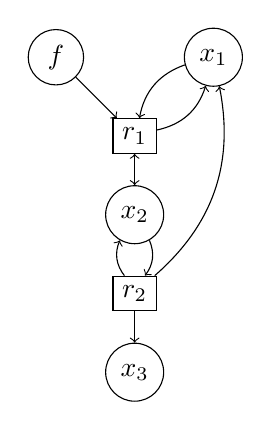
\begin{tikzpicture}
			\node[draw, circle] (f) at (0,0) {$f$};
			\node[draw, circle] (x1) at (2,0) {$x_1$};	
			\node[draw, circle] (x2) at (1,-2) {$x_2$};
			\node[draw, circle] (x3) at (1,-4) {$x_3$};
		
			\node[draw, rectangle] (r1) at (1,-1) {$r_1$};
			\node[draw, rectangle] (r2) at (1,-3) {$r_2$};
		
			\draw[->] (f) to (r1);
			\draw[->] (x1) to [bend right = 30] (r1);
			\draw[->] (r1) to [bend right = 30] (x1);
			\draw[->] (r1) to (x2);
			\draw[->] (x2) to [bend left = 30](r2);
			\draw[->] (r2) to [bend left = 30](x2);
			\draw[->] (x2) to (r1);
			\draw[->] (r2) to (x3);
			\draw[->] (r2) to [bend right = 30] (x1);
		\end{tikzpicture}	
	\end{minipage}%
	\hfill%
	\begin{minipage}[c]{0.23\textwidth}
		\centering
		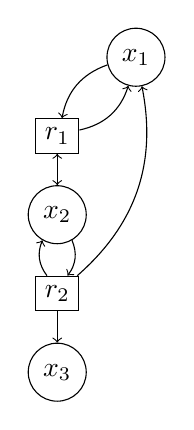
\begin{tikzpicture}
			\node[draw, circle] (x1) at (2,0) {$x_1$};	
			\node[draw, circle] (x2) at (1,-2) {$x_2$};
			\node[draw, circle] (x3) at (1,-4) {$x_3$};
		
			\node[draw, rectangle] (r1) at (1,-1) {$r_1$};
			\node[draw, rectangle] (r2) at (1,-3) {$r_2$};
		
			\draw[->] (x1) to [bend right = 30] (r1);
			\draw[->] (r1) to [bend right = 30] (x1);
			\draw[->] (r1) to (x2);
			\draw[->] (x2) to [bend left = 30](r2);
			\draw[->] (r2) to [bend left = 30](x2);
			\draw[->] (x2) to (r1);
			\draw[->] (r2) to (x3);
			\draw[->] (r2) to [bend right = 30] (x1);
		\end{tikzpicture}	
	\end{minipage}%
	\hfill%
	\begin{minipage}[c]{0.23\textwidth}
		\centering
		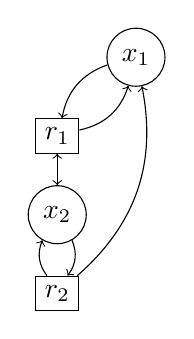
\begin{tikzpicture}
			\node[draw, circle] (x1) at (2,0) {$x_1$};	
			\node[draw, circle] (x2) at (1,-2) {$x_2$};
		
			\node[draw, rectangle] (r1) at (1,-1) {$r_1$};
			\node[draw, rectangle] (r2) at (1,-3) {$r_2$};
		
			\draw[->] (x1) to [bend right = 30] (r1);
			\draw[->] (r1) to [bend right = 30] (x1);
			\draw[->] (r1) to (x2);
			\draw[->] (x2) to [bend left = 30](r2);
			\draw[->] (r2) to [bend left = 30](x2);
			\draw[->] (x2) to (r1);
			\draw[->] (r2) to [bend right = 30] (x1);
		\end{tikzpicture}	
	\end{minipage}
	\caption{A minimal RAF $\RAF$ \textit{(left)} with its directed K\"onig graph represnetation 
	$G\coloneqq \king[\closure{\RAF}{F}, \RAF]$  \textit{(middle left)}, $H\coloneqq \king[\closure{\RAF}{F} 
	\setminus F, \RAF]$ \textit{(middle right)}, and $L\coloneqq H[V(H) \setminus W, \RAF], W 
	\coloneqq \{x\in \closure{\RAF}{F} \ | \ \nexists r \in \RAF \text{ s.t. } s^-_{xr}>0\}$ \textit{(right)}.}
	\label{fig:}
\end{figure}
\FloatBarrier

Indeed, $\{r_1,r_2\}$ is a RAF w.r.t. to $F$. Nevertheless, $x_3$ is never consumed by any reaction. Naturally, any strictly positive reaction 
vector yields a net increase in the concentration of such species, which motivates to consider the graph $H$ without those vertices. In addition, 
these species are never located on an elementary circuit, and we obtain that Lemma~\ref{lem:strElCirc} holds if these species are removed.
\vspace{6pt}
\begin{corollary}\label{lem:strElCirc}
	Let $(X,R, \cat)$ be a catalyzed network with food-set $F$, and $\RAF$ a minimal, non-trivial RAF. Any two elementary circuits $C_1,C_2$ 
	in $L\coloneqq H[V(H)\setminus W]$ with $W\coloneqq \{x\in \closure{\RAF}{F} \ | \ \nexists r \in \RAF \text{ s.t. } s^-_{xr}>0\}$ are strongly connected. 
\end{corollary}
\vspace{6pt}
For brevity of presentation, we let 
\begin{equation}\label{eq:graphL}
	L\coloneqq H[V(H]\setminus W], W\coloneqq \{x\in \closure{\RAF}{F} \ | \ \nexists r \in \RAF \text{ s.t. } s^-_{xr}>0\} 
\end{equation}
in the following. If $\RAF$ is composed of a single reaction, then $L$ is a singleton, i.e., the very reaction vertex of $\RAF$. 
We may therefore directly conclude:


%\vspace{6pt}
%\begin{lemma}\label{lem:weaklyConnected}
%	The graph $\queen'$ is weakly-connected.
%\end{lemma}
%\begin{proof}
%	Assume this is not the case. Then we have at least two connected components $\queen_1', \queen_2'$. By assumption both $X(\queen_1')$ 
%	and $X(\queen_2')$ are $\food$-generated. Since all F-reactions in $\RAF$ are catalyzed, every F-reaction in $\FR(\queen_1')$ and every F-reaction 
%	in $\FR(\queen_2')$ is catalyzed. Since there is no path from any $x_1\in X(\queen_1')$ to any $\fr_2\in \FR(\queen_2')$ and no path from 
%	any $x_2\in X(\queen_2')$ to any $\fr_1\in \FR(\queen_1')$, every F-reaction $\fr_1\in \FR(\queen_1')$ is catalyzed by an $x_1\in X(\queen_1')$ 
%	and every F-reaction of $\fr_2\in \FR(\queen_2')$ is catalyzed by an entity of $x_2\in X(\queen_2')$. In addition, no reaction $\fr_1\in \FR(\queen_1')$ 
%	has a species $x_2\in X(\queen_2')$ as F-reactant and no reaction $\fr_2\in \FR(\queen_2')$ has a species $x_1\in X(\queen_1)$ as F-reactant. 
%	Thus $\FR(\queen_1')$ and $\FR(\queen_2')$ are RAFs themselves. Since $\FR(\queen_1'), \FR(\queen_1')\subseteq \RAF$, $\RAF$ was not minimal.
%\end{proof}
%\vspace{6pt}
%A minimal RAF, thereby, has a corresponding weakly-connected bipartite K\"onig graph, which is also the case for the 
%subgraph that contains only non-food molecules.
%\vspace{6pt}
%\begin{lemma}\label{lem:weaklyConnected2}
%	The subgraph $\queen'' \coloneqq \queen'[\closure{}{\food}\setminus \food, \RAF]$ is weakly-connected.
%\end{lemma}
%\begin{proof}
%	By Lemma~\ref{lem:weaklyConnected}, $\queen'$ is weakly-connected. Assume now there is an $f\in \food$ 
%	such that $\queen'[V(\queen')\setminus \{f\}]$ is composed of at least two connected components $C_1, C_2$. Then 
%	$\closure{\FR(C_1)}{\food}\cap \closure{\FR(C_2)}{\food} \subseteq \food$, i.e., none of the species $x_1\in X(C_1)$ 
%	is a reactant, product, or catalyst for an F-reaction $\fr_2\in \FR(C_2)$ and vice versa. Thus, $\FR(C_1), \FR(C_2)$ 
%	are both RAFs and $\RAF$ was not minimal.
%\end{proof}
%\vspace{6pt}

%\begin{lemma}\label{lem:elemCirc1}
%	Let $\RAF$ be a minimal, non-trivial RAF, with $|\POR^1_{\RAF}(F)|=1$. 
%	Then $r\in \POR^1_{\RAF}(F)$ is located on an elementary circuit that is 
%	not a digon in $G$ and $H$.
%\end{lemma}
%\begin{proof}
%	We show this for $H$ first. Since $\RAF$ is non-trivial $|\RAF|>1$. If $\cat_{r}\subseteq F$ then $\{r\}$ is a minimal RAF.
%	Thus, there is $c\in \cat_r: c\not in F$. Then $c\in D(r)$. If $c\in \cproducts(r)$, then $\{r\}$ again
%	is minimal $\RAF$. With the edge $(c,r)$, $(r,\ldots, c, r)$ is an elementary circuit that is not 
%	a digon. Addition of the food-molecules does not disrupt this argument; thus, the statement 
%	also holds for $G$.	
%\end{proof}
%
%
%\vspace{6pt}
%We now extend this result.
%\vspace{6pt}
%
%\begin{lemma}
%	Let $\RAF$ be a minimal, non-trivial RAF, with $|\POR^1_{\RAF}(F)|=1$. 
%	Then any $r\in \RAF$ is located on an elementary circuit that is 
%	not a digon in $G$ and $H$.
%\end{lemma}
%\begin{proof}
%	Again, we start with the graph $H$. We know that $r_1\in \POR^1_{\RAF}(F)$ is located on 
%	an elementary circuit. Assume now there is a reaction $r\in \RAF$ that is not located on an 
%	elementary circuit. We now show that $\RAF' \coloneqq \RAF\setminus (R(D(r))\cup \{r\}$ 
%	is a RAF. First, we observe that $\RAF'\neq \emptyset$, since $r_1\notin \RAF'$. Otherwise,
%	$r$ would be located on an elementary circuit. Therefore, 	assume $\RAF'$ is not a $\RAF$. 
%	Since $\RAF$ is reflexively autocatalytic and $\RAF'\subseteq \RAF$, $\RAF'$ is reflexively 
%	autocatalytic. Then, there is a reaction $r'\in \RAF'$ for which a reactant or a catalyst $x\in 
%	X(H)$ with $s^-_{xr'}>0$ it holds that $x\notin \closure{\RAF'}(F)$. Since $x\in \closure{\RAF}(F)$ 
%	is a product of some reaction $r''\in R(D(R'))\cup \{r'\}$. However, then $r''\in R(D(R'))\cup \{r'\}$, 
%	which is a contradiction. Thus, $\RAF'$ is a RAF and therefore $\RAF$ was not minimal. Adding
%	the food molecules to $H$ does not change the arguments, thus the result also holds for $G$. 	
%\end{proof}

%\begin{figure}
%	\begin{minipage}[c]{0.5\textwidth}
%		\centering
%		\begin{equation*}
%			\begin{split}
%				r'_0 &: f + (x_1) 		\rightarrow x_2  + (x_1) \\
%				r''_0 &: f + (y_1) 		\rightarrow x_2  + (y_3) \\
%				r_1 &: x_2	+ (x_2)	   	\rightarrow x_1 + y_1 + (x_2) \\
%			\end{split}
%		\end{equation*}
%	\end{minipage}%
%	\hfill%
%	\begin{minipage}[c]{0.49\textwidth}
%		\begin{minipage}[c]{\textwidth}
%			\centering
%			\begin{tikzpicture}
%				\node[draw, circle] (f) at (0,0) {$f$};
%				\node[draw, circle] (x1) at (2,1) {$x_1$};
%				\node[draw, circle] (x2) at (2,0) {$x_2$};
%				\node[draw, circle] (y1) at (2,-1) {$y_1$};
%						
%				\node[draw, rectangle] (r'0) at (1,1) {$r'_0$};
%				\node[draw, rectangle] (r''0) at (1,-1) {$r''_0$};
%				\node[draw, rectangle] (r1) at (3,0) {$r_1$};
%			
%				\draw[->] (f) to (r'0);
%				\draw[->] (f) to (r''0);
%				\draw[->] (x1) to [bend right = 30] (r'0);
%				\draw[->] (r'0) to [bend right = 30] (x1);
%				\draw[->] (y1) to [bend right = 30] (r''0);
%				\draw[->] (r''0) to [bend right = 30] (y1);
%				\draw[->] (r'0) to (x2);
%				\draw[->] (r''0) to (x2);
%				\draw[->] (x2) to [bend right = 30] (r1);
%				\draw[->] (r1) to [bend right = 30] (x2);
%				\draw[->] (r1) to [bend right = 30] (x1);
%				\draw[->] (r1) to [bend left = 30] (y1);			
%			\end{tikzpicture}
%		\end{minipage}
%		\begin{minipage}[c]{\textwidth}
%			\centering
%			\begin{tikzpicture}
%				\node[draw, circle] (f) at (-1,0) {$f$};
%				\node[draw, circle] (x1) at (0,1) {$x_1$};
%				\node[draw, circle] (x2) at (2,0) {$x_2$};
%				\node[draw, circle] (y1) at (0,-1) {$y_1$};
%						
%				\node[draw, rectangle] (r0) at (1,0) {$\fr_0$};
%				\node[draw, rectangle] (r1) at (3,0) {$\fr_1$};
%			
%				\draw[->] (f) to (r0);
%				\draw[->] (x1) to [bend right = 30] (r0);
%				\draw[->] (r0) to [bend right = 30] (x1);
%				\draw[->] (y1) to [bend right = 30] (r0);
%				\draw[->] (r0) to [bend right = 30] (y1);
%				\draw[->] (r0) to (x2);
%				\draw[->] (x2) to [bend right = 30] (r1);
%				\draw[->] (r1) to [bend right = 30] (x2);
%				\draw[->] (r1) to [bend right = 30] (x1);
%				\draw[->] (r1) to [bend left = 30] (y1);			
%			\end{tikzpicture}
%		\end{minipage}
%	\end{minipage}
%\end{figure}
%\FloatBarrier

%The minimality condition has a series of interesting consequences on the structure of the graph $\queen'$.  
%The next one follows from Lemma~\ref{lem:RAFPath}.
%\vspace{6pt}
%\begin{lemma}[Proof: SI]\label{lem:weaklyConnected}
%	The graph $\queen'$ is weakly-connected.
%\end{lemma}
%\vspace{6pt}

%The easiest example of a minimal RAF is a single reaction, which we call a trivial RAF. The following example shows a 
%non-minimal RAF containing a trivial RAF.\\
%\vspace{6pt}
%\begin{minipage}[c]{0.4\textwidth}
%	\centering
%	\begin{equation}
%		\begin{split}
%			r_0&: f_2 + (f_1)\rightarrow x_1 + (f_1)\\
%			r_1&: x_1+ (x_1) \rightarrow x_2 + (x_1)\\
%			r_2&: x_1 + (x_1) \rightarrow x_2 + (x_1)
%		\end{split}
%	\end{equation}
%\end{minipage}%
%\hfill%
%\begin{minipage}[c]{0.55\textwidth}
%	\begin{tikzpicture}
%		\node[draw,circle] (f1) at (0,0) {$f_1$};
%		\node[draw,circle] (f2) at (0,-2) {$f_2$};
%		\node[draw,circle] (x1) at (2,-1) {$x_1$};
%		\node[draw,circle] (x2) at (4,-1) {$x_2$};
%		
%		\node[draw,rectangle] (r0) at (1,-1) {$r_0$};
%		\node[draw,rectangle] (r1) at (3,0) {$r_1$};
%		\node[draw,rectangle] (r2) at (3,-2) {$r_2$};
%		
%		\draw[->] (f1) to [bend left =30] (r0);
%		\draw[->] (f2) to  (r0);
%		\draw[->] (r0) to [bend left =30] (f1);
%		\draw[->] (r0) to (x1);
%		\draw[->] (x1) to [bend right =30] (r1);
%		\draw[->] (r1) to [bend right =30] (x1);
%		\draw[->] (r1) to (x2);
%		\draw[->] (x2) to [bend right =30] (r2);
%		\draw[->] (r2) to [bend right =30] (x2);
%		\draw[->] (r2) to (x1);
%	\end{tikzpicture}
%\end{minipage}
%Indeed, $\RAF=\{\fr_0\}$ is a RAF, and thus, addition of $\fr_1$ or $\fr_2$ would violate minimality. 


%\TODO{Construction site ahead}
%A natural extension to this statemen relies on considering not only species from 
%$\closure{\RAF}{F}\setminus F$ but from the set of food-generated entities, i.e.
%\begin{equation}
%	\mathbf{X}_{\RAF} \coloneqq \bigcup_{k=1}^n \POX^k_{\RAF}(F)
%\end{equation}
%
%However, in this case, semipositivity is not guaranteed. To see this, consider 
%the following example:
%
%\begin{equation}
%	\begin{split}
%		r_1: f_1 & \overset{f_1}{\longrightarrow} x_1\\
%		r_2: x_1 & \overset{x_1}{\longrightarrow} f_1 \\		
%	\end{split}
%\end{equation}
%
%with the RAF $\RAF\coloneqq \{r_1,r_2\}$ and food-set $F\coloneqq \{f_1\}$. Then
%$\SM[\mathbf{X}_{\RAF}, \RAF]$ reads:
%
%\begin{equation}
%	\begin{pmatrix}
%		-1 & 1 \\
%		1 & -1
%	\end{pmatrix}
%\end{equation}
%
%which is indeed not semipositiv. 
%
%Non-trivial minimal RAFs are strongly connected and can be decomposed into strong blocks. 
%The subnetwork induced by each of these strong blocks is naturally well-formed. In addition,
%any species is solely produced or consumed by a reaction within the block. Thereby, the sub-vector
%of $v$ as constructed in the proof of Thm.~\ref{thm:NonFoodSemipositiv} and restricted to the 
%reactions contained in the strong block, directly yields semipositivity on the submatrix containing
%all species and reaction vertices within the strong block.
%
%
%The semipositivity of $A\coloneqq \SM[(\closure{\RAF}{F}\setminus F,\RAF)]$ in general originates 
%from at least one of the form $x_1\rightarrow x_1 + x_2$. For example, in the following RN:
%\begin{equation}
%	\begin{split}
%		r_0: f_1 & \overset{f_2}{\longrightarrow} x_1 \\ 
%		r_i: x_i & \overset{x_i}{\longrightarrow} x_{i+1},
%	\end{split}
%\end{equation}
%reaction $r_0$ forms a non-negative column in $A$, which allows for an unrestricted input of $x_1$. 
%However, $r_0$ has no reactant in $\closure{\RAF}{F}\setminus F$, not even a catalyst. By 
%definition~\ref{def:autSubRN}, $(\closure{\RAF}{F}\setminus F,R')$ is not an autocatalytic subnetwork 
%since it is not well-formed. One way of avoiding such a situation is to require that none of the 
%catalysts is contained in the food set. Consider the following 
%RAF $\RAF={r_1,r_2}$, with food-set $F=\{f\}$ and $X\coloneqq \{f,x_1,x_2\}$.
%\begin{equation}
%	\begin{split}
%		r_1&: f  \overset{x_1}{\longrightarrow} x_2 \\ 
%		r_2&: x_2  \overset{x_2}{\longrightarrow} x_1
%	\end{split}
%\end{equation}
%The matrix $A\coloneqq \SM[(\closure{\RAF}{F}\setminus F,R')]$ then reads:
%\begin{equation}
%	A\coloneqq 
%		\begin{pmatrix}
%			0 & 1\\
%			1 & -1
%		\end{pmatrix}
%\end{equation}
%which is an autocatalytic core of size $2$ that is associated with an elementary 
%circuit in $\king(\closure{\RAF}{F},R'), R')$. This is, however, no coincidence. 
%Let us therefore consider only \emph{catalytically autonomous} RAFs $\RAF$, 
%i.e., for which $\cat(\RAF)\cap F=\emptyset$.
%\vspace{6pt}
%\begin{lemma}
%	Let $(X,R)$ be a catalyzed network with food-set $F$ and $\RAF$ a \emph{catalytically autonomous} RAFs. 
%	Then $(\closure{\RAF}{F},\RAF)$ contains an autocatalytic core $(X',R')$ that is either an explicit autocatalytic 
%	reaction or $\king(X',R')$ is an elementary circuit and the corresponding CS matrix $\SM[\child]$ has at least 
%	one strong Metzler column.
%\end{lemma}
%\begin{proof}
%	\TODO{Include and adapt proof from Overleaf}
%\end{proof}
%\vspace{6pt}
%
%Generalizing this notion, we can require that every reaction has a reactant (not necessarily a net-reactant)
%that is not an element of the food set. 
%
%\begin{lemma}
%	Let $(X,R)$ be a catalyzed network with food-set $F$ and $\RAF$ a RAF, where for each $r\in R'$ there is
%	$x\in \closure{\RAF}{F}\setminus F: s_{xr}^->0$. Then $(\closure{\RAF}{F},\RAF)$ contains an autocatalytic 
%	core $(X',R')$ that is either an explicit autocatalytic reaction or $\king(X',R')$ is an elementary circuit and the 
%	corresponding CS matrix $\SM[\child]$ has at least one strong Metzler column.
%\end{lemma}
%\begin{proof}
%	
%\end{proof}
% 
%Building on this....
%
%\begin{lemma}
%	A RAF is a CAF or it contains an autocatalytic core.
%\end{lemma}
%\TODO{Another open point here is that we can have food molecules that are produced....not entirely sure yet how to 
%deal with this case.}
%
%\vspace{6pt}
%
%\section{RAF-Subnetworks}
%
%In this subsection, we aim to generalize the framework of RAFs to a subnetwork setting.
%
%\subsection{Reflexively autocatalytic subnetworks}
%
%We start with the reflexive-autocatalytic part. We call a subnetwork $(X', R')$ partially catalyzed if $\cat(R')\neq \emptyset$. 
%\vspace{6pt}
%\begin{definition}
%	Let $(X,R)$ be a catalyzed RN. A subnetwork $(X',R')$ is called reflexive-autocatalytic if for each 
%	$r\in R': \cat_r\neq \emptyset \ (X(\cat(R')\subseteq X')$. It is called autonomously reflexive-autocatalytic 
%	if for each $r\in R': \cat_r\neq \emptyset \ and X(\cat(R')\subseteq X'$.
%\end{definition}
%\vspace{6pt}
%We denote the subgraph of a subnetwork by $\king'\coloneqq \king(X',R')$ and write $\cat'$ instead of $\cat(R')$. A direct consequence 
%is the following lemma:
%\vspace{6pt}
%\begin{lemma}\label{lem:RASubnetwork}
%	Let $(X, R, \cat)$ be a catalyzed RN. A subnetwork $(X',R')$ is (autonomously) reflexive-autocatalytic if and only if
%	for all $r\in R' \ \exists x\in X: (x,r),(r,x)\in E(\king(X\cup X(\cat'), R') \ (E(\king'))$. 
%\end{lemma}
%\begin{proof}
%	If $(X',R')$ is reflexive autocatalytic $|R'|=|\cat'|$, thus each reaction $r$ is explicitely catalyzed by an $x_r\in X(\cat_r)\subseteq X$.
%	Then $s^-_{x_rr}>0$ and $s^+_{x_rr}>0$ yields by definition $(x_r,r)$ and $(x_r,r) \in E(\king(X\cup X(\cat'), R')$, respectively.
%	If $(X',R')$ is autonomously reflexive-autocatalytic then $X(\cat'\subseteq X'\Rightarrow \king(X\cup X(\cat'), R') = \king'$ which
%	yields the second part of the claim. Conversely, if for each $r\in R': \exists x\in X$ such that $(x,r),(r,x)\in E(\king(X\cup X(\cat')), R')$, 
%	then by definition $s^-_{xr}>0,s^+_{xr}>0$, thus $x\in X(\cat_r)$. If, additionally, $(x,r),(r,x) \in E(\king')$ then $x\in X'$ and thus 
%	$X(\cat'\subseteq X'$ which yields that $(X',R')$ is autonomously reflexive-autocatalytic. 
%\end{proof}
%\vspace{6pt}
%
%\subsection{F-generated subnetworks}
%
%In theory, for an RN $(X,R,\cat)$, $F$ could be chosen arbitrarily. Depending on the network structure and the RAF $R'$, 
%$F$ might be identical to its own closure. To see this, consider the following example network: 
%\begin{equation}
%	\begin{split}
%		r_1: x_1 \overset{x_1}{\longrightarrow} x_2 \\
%		r_2: x_2 \overset{x_2}{\longrightarrow} x_1 \\
%	\end{split}
%\end{equation}
%with $F=\cat=X=\{x_1,x_2\}$ and RAF $\RAF = \{r_1,r_2\}$. Then $F=\closure{\RAF}{F}$. However, $F$ could also contain reactions 
%that are not connected to the rest, depending on the RAF. For example
%\begin{equation}
%	\begin{split}
%		r_1: x_1 &\overset{x_1}{\longrightarrow} x_2 \\
%		r_2: x_2 &\overset{x_2}{\longrightarrow} x_1 \\
%		r_3: x_3 &\overset{x_3}{\longrightarrow} x_1 
%	\end{split}
%\end{equation}
%with $F=\cat=X=\{x_1,x_2,x_3\}$ and RAF $\RAF=\{r_1,r_2\}$, we have $x_3\in F\Rightarrow F\subseteq \closure{\RAF}{F}$ but $x_3$ is disconnected
%in the graph $\king(X(\RAF) \cup F, \RAF, \cat(\RAF))$. In contrast, a food-set $F'$ for a subnetwork $(X', R')$ as defined in Eq.~\ref{eq:FoodWaste} is a direct 
%consequence from the set of entities $X'$ and the set of reactions $R'$. 
%
%\vspace{6pt}
%\begin{definition}[F-generated subnetwork]
%	Let $(X, R, \cat)$ be a catalyzed RN. A subnetwork $(X',R')$ is called $F$-generated, if $X'\subseteq \closure{R'}{F}$.
%\end{definition}
%\vspace{6pt}
%
%An immediate question that arises is how to construct a minimal set $F$ to obtain an $F$-generated subnetwork. Clearly, we have  
%that $F'\subseteq F$ if $(X',R')$ is $F$-generated. 
%\vspace{6pt}
%\begin{lemma}
%	Let $(X, R, \cat)$ be a catalyzed RN and $(X',R')$ a subnetwork. If $\king[X'\cup R']$ is a fluffle, then $(X',R')$  
%	is an $F$-generated subnetwork for any of the sets $F_x\coloneqq F'\cup\{x\}, x\in X'$.
%\end{lemma}
%\begin{proof}
%	If $\king[X'\cup R']$ is a fluffle, then any reaction has a single reactant in $(X',R')$. In addition, there is a unique CS $\child$ 
%	defined by the reactant-to-product edges. For an arbitrary $x'\in X'$ and the set $F'$ we have $E(\kappa(x))\subseteq 
%	F_x\coloneqq F'\cup\{x\}$, which yields that $P(\kappa(x))\subseteq \cl_{R'}(F_x)$. For all $y\in P(\kappa(x))$, the same 
%	argument applies as well as for all any $z\in \POX^k_{R'}(F), k\leq n$. Since $\king[X'\cup R']$ is a fluffle, it is strongly 
%	connected. Thus, for each $r\in R'$ there is path $(x, \kappa(x), \ldots, r)$, and thereby an $k\leq n: r\in \POR_{R'}(F)$. 
%	Hence, $X'\subseteq \closure{R'}{F}$.
%\end{proof}
%\vspace{6pt}
%Since irreducible Metzler CS matrices have a bipartite graph representation as a fluffle, 
%the following statement is a direct consequence from the former lemma.
%\vspace{6pt}
%\begin{corollary}
%	Let $(X',R')$ be a subnetwork that has an associated autocatalytic, irreducible 
%	Metzler CS matrix $\SM[\child]$. Then $(X',R')$ is an $F$-generated
%	subnetwork for any $F_x\coloneqq F'\cup \{x\}, x\in X'$.
%\end{corollary}
%\vspace{6pt}
%Any autocatalytic core $(X',R')$ can then be generated by the union of $F'$ and a single species from $X'$. 
%\vspace{6pt}
%\begin{corollary}
%	Let $(X',R')$ be an autocatalytic core. Then $(X',R')$ is an $F$-generated subnetwork for any $F_x\coloneqq F'\cup \{x\}, x\in X'$.
%\end{corollary}
%\vspace{6pt}
%For irreducible non-Metzler matrices, such a result cannot be obtained. In the worst case, 
%all but one species might have to be added to $F'$ to obtain an $F$-generated subnetwork. 
%To see this, consider the following subnetwork $(X',R')$: 
%\begin{equation}
%	\begin{split}
%		r_1&: x_1 + \epsilon x_3 \rightarrow x_2 \\
%		r_2&: x_2 + \epsilon x_1 \rightarrow x_3 \\
%		r_3&: x_3 + \epsilon x_2 \rightarrow x_1
%	\end{split}
%\end{equation}
%with corresponding CS matrix:
%\begin{equation}
%	\SM[\child]=\begin{pmatrix}
%				-1 & -\epsilon & 2 \\
%				1 & -1 & -\epsilon \\
%				-\epsilon & 1 & -1 
%			\end{pmatrix}
%\end{equation}
%which is autocatalytic for epsilon small enough with $v=\begin{pmatrix}5 & 4 & 3\end{pmatrix}^T$. 
%In \cite{golnik_enumeration_2025}, it has been shown that any CS matrix with irreducible Metzler has a 
%spanning fluffle $\king(\child)$. Although still strongly connected the induced subgraph $\king[\child]$ 
%might contain additional reactant-to-reaction edges that are not encoded by the CS-bijection $\kappa$.
%However, it is sufficient to add all species with an off-diagonal entry.
%\vspace{6pt}
%\begin{lemma}
%	Let $(X', R')$ be a subnetwork with a non-Metzler CS matrix with irreducible Metzler part. Then $(X',R')$
%	is $F$-generated for $F= F' \cup N, N=\{x\in X' | \exists r \neq \kappa(x), \SM^-_{xr}>0\}$.
%\end{lemma}
%\begin{proof}
%	Since $\SM[\child]$ has irreducible Metzler part, $\king(\child)$ is strongly-connected, which implies that
%	also $\king[\child]$ is strongly connected. Then for any $x\in N: E(\kappa(x))\in F$, thus $\kappa(x)\in \POR_{R'}(F)$ 
%	and $P(\kappa(x))\in \cl_{R'}(F)$. We can now recursively apply this argument to all $y\in P(\kappa(x))$
%	and obtain with the strong-connectedness of $\king[\child]$ that $X'\subseteq \closure{R'}(F)$.
%\end{proof}
%\vspace{6pt}
%%\subsection{Reflexively autocatalytic and $F$-generated subnetworks}
%%
%%We now combine the two definitions above. 
%%
%%\begin{definition}
%%	Let $(X, R, \cat)$ be a catalyzed RN and $(X',R')$ a subnetwork. A reflexive autocatalytic subnetwork $(X',R')$ 
%%	is called a RAF-subnetwork if there is a set $Y'\subseteq X'$ such that $(X',R')$ is $F$-generated for $F\coloneqq F'\cup Y'$.
%%\end{definition}
%%
%%%A trivial statement that follows directly from the definition is that for any RAF subnetwork
%
%\vspace{6pt}
%The definition of the food-set $F'$ in Eq.~\ref{eq:FoodWaste} does not include catalysts. We may additionally define the catalyst 
%specific food-set for $(X',R')$ as follows:
%\begin{equation}
%	F'_{\cat'}\coloneqq \{x\in X(\cat') \ | \ x\notin X'\} 
%\end{equation}


\end{document}